\documentclass[conference]{IEEEtran}

\usepackage[pdftex]{graphicx}
\usepackage[utf8]{inputenc} % Diacritics and special letters.
\usepackage[T1]{fontenc} % Encoding table for characters.
\usepackage{flushend}

\begin{document}

%-------------------------------------------------------------------------
\title{Simulation Platform for Wired/Wireless Networks with Mixed Time and Reliability Requirements}
%-------------------------------------------------------------------------

%TODO other possible tiles
% Simulation Platform and Scenario Generator for Time-Triggered Wired/Wireless Networks
% Simulation Platform and Scenario Generator for Wired/Wireless Networks with Mixed Time and Reliability Requirements

%TODO other possible title wordings
% -Simulation
% -Platform, toolchain, environment
% -Time-triggered, TDMA, mixed-traffic requirements
% -Ethernet-based
% -Hybrid, wired/wireless networks
% -Scenarios generation

\author{
\IEEEauthorblockN{Pablo Gutiérrez Peón\IEEEauthorrefmark{1}\IEEEauthorrefmark{2},
Francisco Pozo\IEEEauthorrefmark{2}}

\IEEEauthorblockA{\IEEEauthorrefmark{1}TTTech Computertechnik AG, Vienna, Austria}

\IEEEauthorblockA{\IEEEauthorrefmark{2}School of Innovation, Design and Engineering, Mälardalen University, Västerås, Sweden\\
Email: pablo.gutierrez-peon@tttech.com, francisco.pozo@mdh.se}}

\maketitle

%-------------------------------------------------------------------------
\begin{abstract}
%-------------------------------------------------------------------------

The use of computer simulations can help to evaluate the performance of real-time data networks and detect potential issues that compromise the ultimate goal of providing timely and reliable communications. A theoretical analysis over components of the communication system such as the physical layer, medium access, or routing, is many times too complex or only able to cover pessimistic cases. Further, real-time data communication technologies often make use of wired links, where problems like fading, shadowing or interference are not generally as crucial as in wireless links. Still, advantages like mobility, flexibility in the deployment or reduced cost and weight might trigger the consideration of wireless communications. Instead of completely replacing wired links, wireless links are often seen as a complement to wired networks, enabling new application domains. At the same time, there is a trend towards the convergence between networks for industrial, automotive or aerospace fields serving real-time requirements and networks for office and home environments that focus on throughput at the cost of offering a best-effort service. Important to mention is that message scheduling is crucial in the design of a real-time communication systems. Unlike event-triggered message dispatching, in the time-triggered paradigm the instants when transmissions are done are pre-defined, having the advantage that the behaviour of scheduled message transmissions is unique. Unfortunately, accessing the medium does not guarantee that the message will be delivered. Although absolute guarantees cannot be given, simulation can help to evaluate if sufficient reliability is provided for the transmissions and if the timing requirements can be kept.

This work aims at providing a simulation platform to test hybrid wired/wireless networks where both real-time and non-real-time traffic travel seemingly over different transmission media. The simulation platform proposed in this work consists of four main components: network and traffic generator, traffic scheduler, network simulator and results processing. To interface between components, every component takes a file or set of files as an input and generates a set of files as an output.

The network and traffic generator... [Pablo to Francisco: I need you to say something about topology and name the 4 types of devices so that I can refer it below]

The traffic scheduler... [Pablo to Francisco: say that we use FIFO queues?]

The network simulator is developed in the OMNeT++ discrete event simulation framework. The basic components of an OMNeT++ simulation are the modules, the pieces where the functionality is implemented. Modules are connected to each other using gates and exchange information using message passing. The modules are partially described using the NED language from OMNeT++, that specifies the parameters, gates and nested modules, while the functionality is programmed in C++. The initialization file is used to give value to the module parameters. The values can be grouped with labels that define different configurations, each specifying a set of values for the module parameters. The four types of network devices are able to dispatch messages in a time-triggered manner (following the link schedule and frame paths files). The devices are based on IEEE 802.3 and IEEE 802.11 with a modified medium access control (MAC) layer. Inside the MAC, queues are FIFO, and traffic of different classes is segregated into different queues. [say something more about interference, etc.] The simulation can run with a graphical environment or using the command line. The results are provided in three types of files. Scalar and vectorial result files retrieve statistics and vectors of raw data, including, e.g., number of packets sent and received or the instants when those packets are sent. The log file includes entries about relevant events and the time at which they happened.

The results processing...

In order to facilitate the use of the simulation tool, a single file records all the parameters required by the user. To build the set of tools and run them, a makefile is created.

%TODO Motivation:
% - IT/OT, time-triggered, industrial networks

%TODO what do we offer:
% - Hybrid wired/wireless networks
% - Generates traffic and network topologies (describe how)
% - Built-in SMT traffic scheduler.
% - Network simulation. INI file can be modified to tune all the desired parameters.
% - Log checker tool.
% - TT traffic and BE
% - Wireless interferers
% - Reliability, delays (schedule is supposed to work, but here we check it)
% - Mechanisms for improved reliability (retransmissions, cognitive radio
% - Simulation made easy: one input file to generate several tests. Makefile: one instruction and wait for the results.

%TODO Describe the components of the simulator.

%TODO Describe what we have been able to achieve so far? I dont think we can use references.


\end{abstract}

%TODO Make intro to the figures?

%TODO maybe add legend here
\begin{figure*}[h]
	\centerline{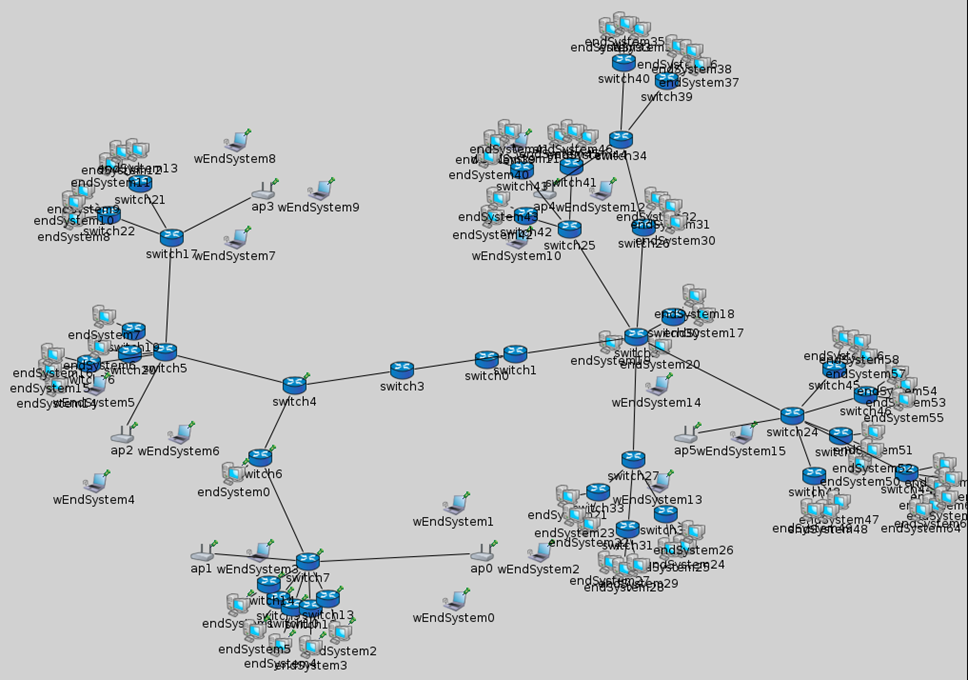
\includegraphics[keepaspectratio=true, width=16cm] {figures/s1-3}}
	\caption{}
	\label{fig:s1-3}
\end{figure*}

\begin{figure*}[h]
	\centerline{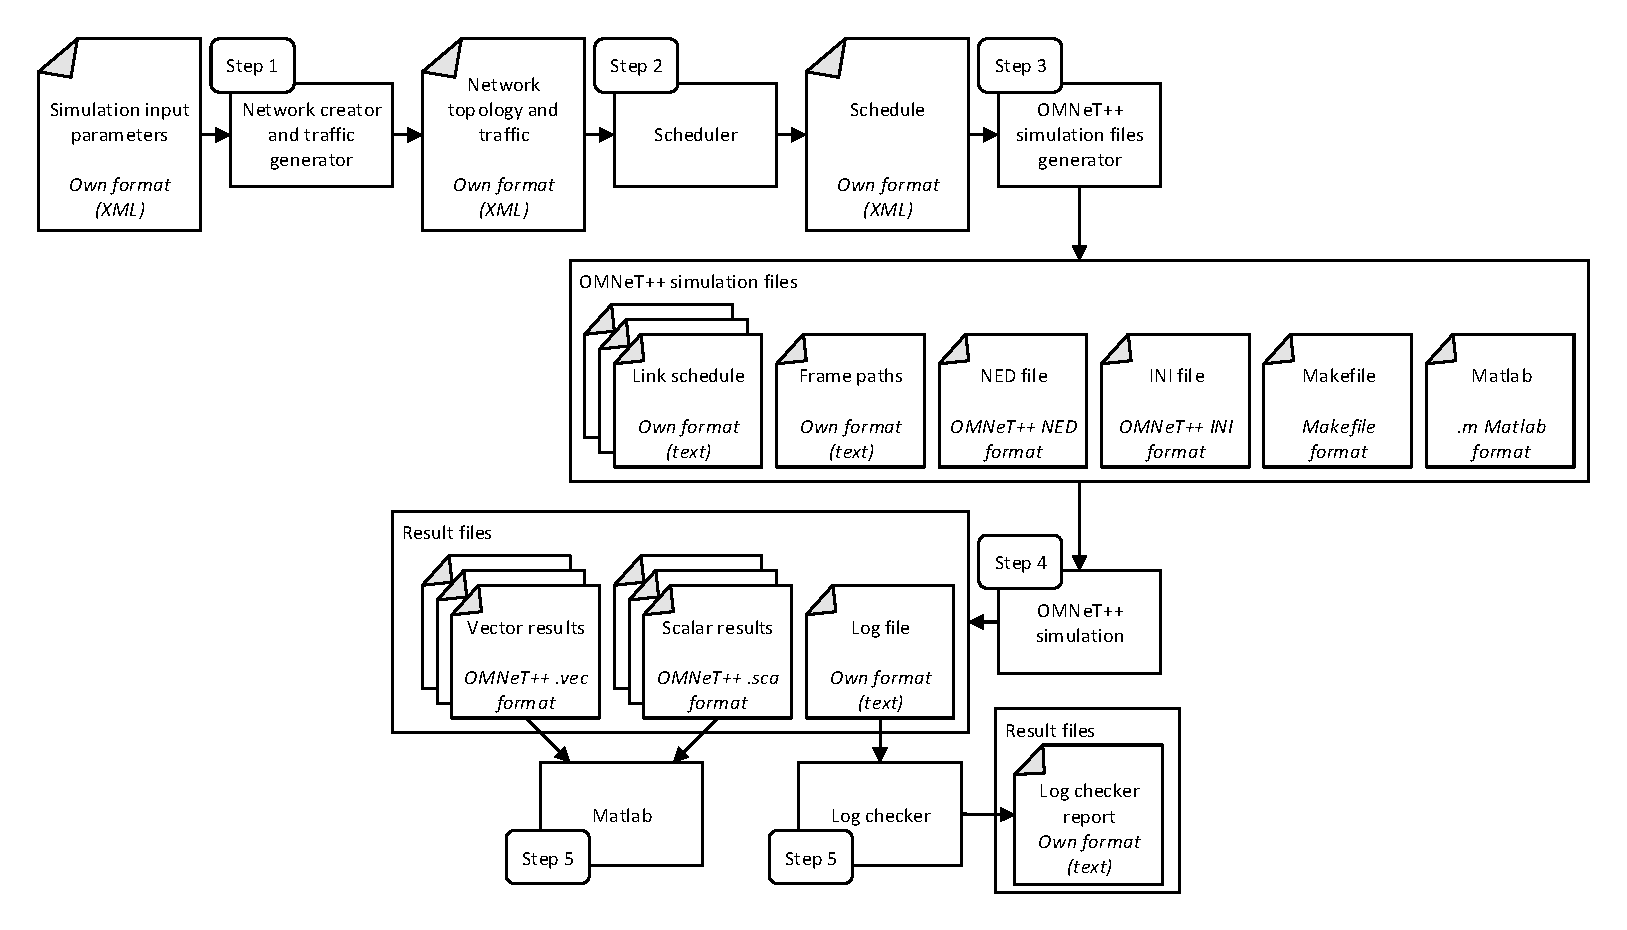
\includegraphics[keepaspectratio=true, width=16cm] {figures/toolchain-architecture}}
	\caption{}
	\label{fig:toolchain-architecture}
\end{figure*}

\end{document}
